\documentclass[authoryear, review, 11pt]{elsarticle}

\setlength{\textwidth}{6.5in}
%\setlength{\textheight}{9in}
\setlength{\topmargin}{0in}
\setlength{\oddsidemargin}{0in}
\setlength{\evensidemargin}{0in}

\usepackage{amsmath}
\usepackage{amsthm}
\usepackage{amssymb}
\usepackage{mathabx}
\usepackage{bm}
\usepackage{multirow}

%\geometry{landscape}                % Activate for for rotated page geometry
\usepackage[parfill]{parskip}    % Activate to begin paragraphs with an empty line rather than an indent
\usepackage{graphicx}
\usepackage{epstopdf}
\usepackage{natbib}
\usepackage{verbatim}
\usepackage{longtable}
\usepackage{rotating}
\usepackage[nolists,nomarkers]{endfloat}
\DeclareDelayedFloatFlavour{sidewaystable}{table}

\usepackage{relsize}
%\usepackage{caption}
\usepackage{subcaption}
\usepackage{fullpage}
\usepackage{booktabs}


\usepackage{setspace}
\setstretch{2}

\DeclareGraphicsRule{.tif}{png}{.png}{`convert #1 `dirname #1`/`basename #1 .tif`.png}
\DeclareMathOperator*{\argmin}{\arg\!\min}
\DeclareMathOperator*{\argmax}{\arg\!\max}
\DeclareMathOperator*{\bw}{\mbox{bw}}
\DeclareMathOperator*{\df}{\mbox{df}}
\newcommand{\vect}[1]{\bm{#1}}
\newcommand{\E}{\mathop{\mathbb E}}






\title{Local Variable Selection and Parameter Estimation of Spatially Varying Coefficient Regression Models}
\author{Wesley Brooks}
\date{}                                           % Activate to display a given date or no date


\begin{document}

\begin{abstract}
The geographically weighted elastic net (GWEN) is introduced as a method for local model selection and coefficient estimation in spatially varying coefficient regression (SVCR) models. Spatially varying coefficient regression is a method of regression analysis for spatial data that allows the regression coefficients to vary across the spatial domain

Geographically weighted regression (GWR) is a kernel-based method for estimating the local regression coefficients in a SVCR model. At each model point a local GWR model is fitted by local likelihood, wherein each observation is weighted based on its location relative to the model point. The GWEN minimizes an objective consisting of a penalty of the elastic net type added to (minus two times) the local likelihood, with the local elastic net tuning parameter selected via the BIC.

The kernel that assigns weight to each observation based on its distance from the model point is governed by a bandwidth parameter. In the GWEN, the bandwidth is a global (as opposed to local) parameter. The bandwidth parameter is selected via the corrected AIC.

Simulations are used to evaluate the performance of the GWEN in model selection and coefficient estimation, and the method is applied to a real data example.
\end{abstract}

\maketitle
%\section{}
%\subsection{}

%Pastebin:
%Spatial association - meaning that nearby locations are more alike than distant locations - is a key concept in spatial statistics.\
%for univariate output $y$, $p$-vector of covariates $\bm{x}$, and random noise $\varepsilon$ all indexed by location $\bm{s}
%where $\phi$ is a bandwidth parameter and $\delta(\bm{s}, \bm{t})$ is the Euclidean distance between locations $\bm{s}$ and $\bm{t}$.

%\begin{spacing}{2}
\section{Introduction}
	%Varying coefficient regression
	Whereas the coefficients in traditional linear regression are scalar constants, the coefficients in a varying coefficient regression (VCR) model are functions - often \emph{smooth} functions - of some effect modifying variable \citep{Hastie:1993a}. When the effect modifying variable represents location in a spatial domain, a VCR model implies a spatially varying coefficient regression (SVCR) model wherein that the regression coefficients vary over space. Statistical inference for the coefficients as functions of location in an SVCR model is more complicated than estimating the coefficients in a traditional linear regression model where the coefficients are constant across the spatial domain. My research concerns the development of new methodology for the analysis of spatial data using SVCR.
	
	%Spatial data / spatial regression
	The methodology described herein is applicable to geostatistical data and areal data. Let $\mathcal{D}$ be a spatial domain on which data is collected. For geostatistical data, let $\bm{s}$ denote a location in $\mathcal{D}$. Let a univariate spatial process $\left\{Y(\bm{s}) : \bm{s} \in \mathcal{D}\right\}$ and a possibly multivariate spatial process $\left\{\bm{X}(\bm{s}) : \bm{s} \in \mathcal{D}\right\}$ denote random fields of the response and the covariates, respectively. For $i = 1, \dots, n$, let $\bm{s}_i$ denote the sampling location in $\mathcal{D}$ of the $i$th observation of the response and the covariates. Let the observed data be denoted $\left\{y(\bm{s}_i), \bm{x}(\bm{s}_i)\right\}$, $i=1, \dots, n$. Then the data are a realization of the random fields at the sampling locations $\left\{Y(\bm{s}_i), \bm{X}(\bm{s}_i)\right\}$ for $i=1, \dots, n$.
	
	For areal data, the spatial domain $\mathcal{D}$ is partitioned into $n$ regions $\{D_1, \dots, D_n\}$ such that $\mathcal{D} = \bigcup \limits_{i=1}^nD_i$. In the case of areal data, the random variables $\left\{Y(D_i), \bm{X}(D_i)\right\}$ are defined for regions instead of for point locations; population and spatial mean temperature are examples of areal data. The analytical method described herein can be applied to areal data if they are recast as geostatistical data by assuming that the data are point-referenced to a representative location of each region, such as the centroid. That is, $\left\{\bm{X}(\bm{s}_i), Y(\bm{s}_i)\right\} $ where $\bm{s}_i$ is the centroid of $D_i$ for $i=1, \dots, n$.
	
	 Common practice in the analysis of geostatistical and areal data is to model the response variable with a spatial linear regression model consisting of the sum of a fixed mean function, a spatial random effect, and random error all on domain $\mathcal{D}$, as in: 
\begin{align}\label{eq:spatial-regression}
    Y(\bm{s}) = \bm{X}(\bm{s})'\bm{\beta} + W(\bm{s}) + \varepsilon(\bm{s})
\end{align}
where $\bm{X}(\bm{s})'\bm{\beta}$ is the mean function consisting of a vector of covariates $\bm{X}(\bm{s})$, and a vector of regression coefficients $\bm{\beta}$. The random error $\varepsilon(\bm{s})$ denotes white noise such that the errors are independent and identically distributed with mean zero and variance $\sigma^2$, while the random component $W(\bm{s})$ denotes a mean-zero, second-order stationary random field that is independent of the random error. The mean function captures the large-scale systematic trend of the response, the spatial random field $W(\bm{s})$ can be thought of as a small-scale spatial random effect, and the error term $\varepsilon(\bm{s})$ captures micro-scale variation \citep{Cressie:1993}.

It is common to pre-specify the form of a covariance function for the spatial random effect $W(\bm{s})$ \citep{Diggle:2007}. For example, the exponential covariance function (a special case of the Mat\'{e}rn class of covariance functions) has the form
\begin{align}\label{eq:exponential-covariance}
    \text{Cov}(W(\bm{s}), W(\bm{t})) = \exp\left\{-\phi^{-1} \delta(\bm{s}, \bm{t}) \right\}
\end{align}
where $\phi$ denotes a range parameter and $\delta(\bm{s}, \bm{t})$ denotes the Euclidean distance between locations $\bm{s}$ and $\bm{t}$. The general form of a covariance function in the Mat\'{e}rn class is
\begin{align}\label{eq:matern-covarinace}
    \text{Cov}(W(\bm{s}), W(\bm{t})) = \left\{\Gamma(\nu) 2^{\nu-1} \right\}^{-1} \left\{\delta(\bm{s}, \bm{t}) \phi^{-1}\sqrt{2\nu}\right\}^\nu K_{\nu} \left(\delta(\bm{s}, \bm{t}) \phi^{-1}\sqrt{2\nu}\right)
    \end{align}
where $\nu$ denotes the degree of smoothness, $K_{\nu}$ denotes the modified Bessel equation of the second kind, and as before $\phi$ denotes a range parameter and $\delta(\bm{s}, \bm{t})$ the Euclidean distance between locations $\bm{s}$ and $\bm{t}$. The exponential covariance function corresponds to a Mat\'{e}rn class covariance function with $\nu = 1/2$.

	%SVCR - justification
	%Stationarity in spatial linear regression
	A random field is said to be stationary if the joint distribution of a the response at a finite set of locations does not change when the set of locations are all shifted in space by a fixed spatial lag. That is, letting $\left\{T(\bm{s}) : \bm{s} \in \mathcal{D}\right\}$ be a random field on spatial domain $\mathcal{D}$ that takes value $T(\bm{s}_i)$ at location $\bm{s}_i \in \mathcal{D}$ for $i = 1, \dots, n$, the random field $T(\bm{s})$ is stationary if $F_n\left(T(\bm{s}_1), \dots, T(\bm{s}_n)\right) = F_n\left(T(\bm{s}_1+\bm{h}), \dots, T(\bm{s}_n+\bm{h})\right)$ where $F_n(\cdot)$ is the joint distribution of a length $n$ sample from $T(\bm{s})$ and $\bm{h}$ is a fixed spatial lag. A random field is second-order stationary if the joint distribution at any two locations in the domain does not change when the locations are shifted by a fixed spatial lag.
	
	The coefficient vector $\bm{\beta}$ in (\ref{eq:spatial-regression}) is a fixed constant. The model can be made more flexible if the coefficients are described by a stationary random field. Such a model is written
\begin{align}\label{eq:SVCR-process}
    Y(\bm{s}) = \bm{X}(\bm{s})'\bm{\beta}(\bm{s}) + \varepsilon(\bm{s})
\end{align}
	where $\bm{\beta}(\bm{s})$ is a random coefficient field with a Mat\'{e}rn-class covariance function and the spatial random effect $W(\bm{s})$ included in the intercept $\beta_0(\bm{s})$. The random coefficient field $\bm{\beta}(\bm{s})$ can be estimated by Markov Chain Monte Carlo (MCMC) methods under the assumption that $\bm{\beta}(\bm{s})$ is stationary \citep{Gelfand:2003}.

	%The spatial random effect describes the spatial pattern in the deviations from the systematic part of the model. When fitting the spatial regression model (\ref{eq:spatial-regression}), it is usually required that the the fitted values of the spatial random effect and of the residuals sum to zero, i.e. $\sum\limits_{i=1}^n\hat{W}(\bm{s}_i) = 0$ and $\sum\limits_{i=1}^n\hat{\varepsilon}(\bm{s}_i) = 0$. This mode of analysis is appropriate when the systematic part of the regression model does not vary between locations. On the other hand, a VCR model is appropriate for the case where the systematic part of the regression model does vary across locations.

	%Spatial VCR
	Alternatively, kernel-based and spline-based methods can be considered for fitting VCR models without assuming the coefficients are described by a stationary random field. For example, it is straightforward to modify a thin plate regression spline model into a traditional, non-spatial VCR model \citep{Wood:2006}. A local likelihood can also be used to fit generalized linear models with varying coefficients using kernel smoothing \citep{Loader:1999}. \cite{Fan:1999} demonstrated that the optimal kernel bandwidth estimate for a VCR model can be found via a two-step technique.
	
	Model selection in VCR models may be local or global. Global selection means including or excluding variables everywhere in the spatial domain, while local selection means including or excluding variables at individual locations within the spatial domain. For global model selection in spline-based VCR models, \cite{Wang:2008a} proposed a SCAD penalty \citep{Fan:2001} for variable selection in spline-based VCR models with a univariate effect-modifying variable. \cite{Antoniadis:2012a} used the nonnegative Garrote penalty \citep{Breiman:1995} in P-spline-based VCR models having a univariate effect-modifying variable.
	
	Wavelet methods for fitting SVCR models were explored by \cite{Shang-2011} and \cite{Zhang-2011}. Sparsity in the wavelet coefficients is achieved either by $\ell_1$-penalization (also known as the Lasso \citep{Tibshirani:1996}) \citep{Shang-2011} or by Bayesian variable selection \citep{Zhang-2011}. Sparsity in the wavelet domain does not imply sparsity in the covariates, though, so neither method is suitable for local variable selection.

	%GWR
	Geographically weighted regression (GWR) is a kernel-based method for estimating the coefficients of an SVCR model where the kernel weights are based on the distance between sampling locations \citep{Brundson:1998a, Fotheringham:2002}. At each sampling location, traditional GWR estimates the local regression coefficients by the local likelihood \citep{Loader:1999}. As a kernel-based smoother for regression coefficients, traditional GWR tends to exhibit bias near the boundary of the region being modeled \citep{Hastie:1993b}. One way to reduce the boundary-effect bias is to model the coefficient surface as locally linear rather than locally constant by including coefficient-by-location interactions \citep{Wang:2008b}.
	
	%Local variable selection
	Traditional GWR relies on \emph{a priori} global model selection to decide which variables should be included in the model. The idea of using Lasso regularization for local variable selection in a GWR model appears in the literature as the geographically weighted Lasso (GWL) \citep{Wheeler:2009}. The GWL applies the Lasso for local variable selection and uses a jackknife criterion for selection of the Lasso tuning parameters. Because the jackknife criterion can only be computed at sampling locations where the response variable is observed, the GWL cannot be used to impute missing values of the response variable nor to interpolate the coefficient surface and/or the response variable between sampling locations.
	
	Lasso regularization for model selection, while popular, can leave relevant covariates out of the model when they are correlated with other covariates, and the predictive performance of the Lasso may be dominated in such a case by ridge regression, which does not allow for local model selection \citep{Tibshirani:1996}. The elastic net is a regularization method that combines a $\ell_1$ (Lasso) and a $\ell_2$ (ridge) penalty on the estimated coefficients, overcoming these drawbacks of the Lasso \citep{Zou:2005}.
	
	Additionally, Lasso regularization does not generally produce consistent estimates of the relevant covariates \citep{Leng-2006}. The adaptive Lasso (AL) \citep{Zou:2006} is an improvement to the Lasso that does produce consistent estimates of the coefficients and has been shown to have appealing properties for automating variable selection, sometimes including the ``oracle" property of asymptotically selecting exactly the correct set of covariates for inclusion in a regression model.
	
	Combining these improvements to the Lasso, the adaptive elastic net (AEN) achieves an oracle property and performs better than other oracle-like methods when there is collinearity in the covariates \citep{Zou:2009}.
	
	This document introduces a new regularization method, called the geographically weighted elastic net (GWEN), for local variable selection in GWR models. Model selection under the GWEN uses the AEN. A penalized-likelihood criterion is used to select the local GWEN tuning parameters, which means that a GWEN can be fit at any location within the domain, whether or not data were observed at that location. The particular information criterion used to select the GWEN tuning parameters is a type of local BIC, but in principle another information criterion like the AIC is also possible. The local BIC presented here is based on the local likelihood \citep{Loader:1999}.
	
	The remainder of this document is organized as follows. The traditional GWR is presented in Section \ref{section:GWR}. The new GWEN is introduced in section \ref{section:model-selection}. In Section \ref{section:simulation}, a simulation study is conducted to assess the performance of the GWEN in variable selection and coefficient estimation. An application of the GWEN to real data is presented in Section \ref{section:data-analysis}. Planned future improvements to the GWEN are discussed in Section \ref{section:future-work}.

\section{Geographically Weighted Regression \label{section:GWR}}
	\subsection{Model}	
	Consider $n$ data observations, taken at sampling locations $\bm{s}_1, \dots, \bm{s}_n$ in a spatial domain $D \subset \mathbb{R}^2$. For $i = 1, \dots, n$, let $y(\bm{s}_i)$ and $\bm{x}(\bm{s}_i)$ denote the univariate response variable, and a $(p+1)$-variate vector of covariates measured at location $\bm{s}_i$, respectively. At each location $\bm{s}_i$, assume that the outcome is related to the covariates by a linear model where the coefficients $\bm{\beta}(\bm{s}_i)$ may be spatially-varying and $\varepsilon(\bm{s}_i)$ is random error at location $\bm{s}_i$. That is,
	\begin{align}\label{eq:lm(s)}
		y(\bm{s}_i) = \bm{x}(\bm{s}_i)' \bm{\beta}(\bm{s}_i) + \varepsilon(\bm{s}_i).
	\end{align}
	
	Further assume that the error term $\varepsilon(\bm{s}_i)$ is normally distributed with zero mean and variance $\sigma^2$, and that $\varepsilon(\bm{s}_i)$, $i=1, \dots, n$ are independent. That is,
	\begin{align} \label{eq:err}
		\varepsilon(\bm{s}_i) \overset{iid}{\sim} \mathcal{N} \left( 0,\sigma^2 \right).
	\end{align}
	
	In order to simplify the notation, let $\bm{x}(\bm{s}_i) \equiv \bm{x}_i \equiv \left( 1, x_{i1}, \dots, x_{ip} \right)'$, $\bm{\beta}(\bm{s}_i) \equiv \bm{\beta}_i \equiv \left(\beta_{i0}, \beta_{i1}, \dots, \beta_{ip} \right)'$, and $y(\bm{s}_i) \equiv y_i$.  Equations (\ref{eq:lm(s)}) and (\ref{eq:err}) can now be rewritten as
	\begin{align}
		y_i = \bm{x}'_i \bm{\beta}_i + \varepsilon_i \text{ and } \varepsilon_i \overset{iid}{\sim} \mathcal{N} \left( 0,\sigma^2 \right).
	\end{align}
	
	Further, let $\bm{X} = \left( \bm{x}_1, \dots, \bm{x}_n \right)'$ and $\bm{y} = \left( y_1, \dots, y_n \right)'$. Thus, conditional on the design matrix $\bm{X}$, observations of the response variable at different locations are independent of each other. Then, a total log-likelihood of the observed data is the sum of the log-likelihood of each individual observation:
	 \begin{align}
	 	\ell\left( \bm{\beta} \right) = - \left(1/2\right) \left\{ n \log \left( 2 \pi \sigma^2\right) +  \left(\sigma^{2}\right)^{-1}  \sum_{i=1}^n \left(y_i - \bm{x}'_i\bm{\beta}_i \right)^2  \right\}.
	\end{align}
	
	Since there are a total of $n \times (p+1)$ free parameters for $n$ observations, the model is not identifiable and it is not possible to directly maximize the total likelihood. One way to effectively reduce the number of parameters is to assume that the coefficients $\bm{\beta}(\bm{s})$ are smoothly varying over space, and use a kernel smoother to make pointwise estimates of the coefficients by maximizing a local likelihood. In the setting of spatial data and with the kernel smoother based on the physical distance between sampling locations, this is the traditional GWR.
		
	\subsection{Estimation}		
	In the traditional GWR, the coefficient surface $\bm{\beta}(\bm{s})$ is estimated at each sampling location $\bm{s}_i$. First calculate the Euclidean distance $\delta_{ii'} \equiv \delta\left(\bm{s}_i, \bm{s}_{i'}\right) \equiv \|\bm{s}_i  -\bm{s}_{i'}\|_2$ between locations $\bm{s}_i$ and $\bm{s}_{i'}$ for all $i, i' = 1, \dots, n$. The bisquare kernel can be used to generate spatial weights based on the Euclidean distances and a bandwidth parameter $\phi$:
	
	\begin{align}\label{eq:bisquare}
		w_{ii'} = \begin{cases} \left\{1-\left(\phi^{-1}\delta_{ii'}\right)^2\right\}^2 &\mbox{ if } \delta_{ii'} < \phi, \\ 0 &\mbox{ if } \delta_{ii'} \geq \phi. \end{cases}
	\end{align}
	
	The bisquare kernel in (\ref{eq:bisquare}) assigns the maximum weight of one where $\bm{s}_i = \bm{s}_{i'}$ (i.e. $\delta_{ii'}=0$), is continuously differentiable, and assigns zero weight to observations at distances greater than one bandwidth from $\bm{s}_i$. For the purpose of estimation, define a local likelihood at each sampling location:
	\begin{align}\label{eq:local-likelihood}
		\mathcal{L}_i \left(\bm{\beta}_i \right) &= \prod_{i'=1}^n \left[ \left(2 \pi \sigma^2_i  \right)^{-1/2}  \exp\left\{-\left(2 \sigma^2_i\right)^{-1}  \left(y_{i'} - \bm{x}'_{i'} \bm{\beta}_i \right)^2 \right\} \right] ^ {w_{ii'}},
	\end{align}			
	where $\sigma_i^2$ is a local approximation to the error variance $\sigma^2$ \citep{Fotheringham:2002}. Thus, the local log-likelihood function is, up to an additive constant:
	\begin{align}\label{eq:local-log-likelihood}
		\ell_i\left(\bm{\beta}_i\right) &= -(1/2) \sum_{i'=1}^n w_{ii'} \left\{ \log{\sigma^2_i}  + \left(\sigma^2_i\right)^{-1}  \left(y_{i'} - \bm{x}'_{i'} \bm{\beta}_i \right)^2 \right\}.
	\end{align}
	From (\ref{eq:local-likelihood}) and (\ref{eq:local-log-likelihood}), it is apparent that the GWR coefficient estimates $\hat{\bm{\beta}}_{i,\text{GWR}}$ maximizing the local likelihood at location $\bm{s}_i$ can be obtained using weighted least squares. 
	
	 Setting to zero the derivative of (\ref{eq:local-log-likelihood}) with respect to $\sigma_i^2$, the maximum likelihood estimate (MLE) $\hat{\sigma}_i^2$ is found to be:	 
	 \begin{align}
	 	\hat{\sigma}_i^2 = \left(\sum \limits_{i'=1}^{n} w_{ii'} \right)^{-1} \sum \limits_{i'=1}^n w_{ii'}\left(y_{i'} - \bm{x}_{i'}'\hat{\bm{\beta}}_i\right)^2
	\end{align}
	
	\begin{comment}
	\paragraph{Algorithmic details} Both $\hat{\bm{\beta}_i}$ and $\hat{\sigma}_i^2$ can be obtained by the method of least squares. Let $\bm{W}_i$ denote a diagonal weight matrix with diagonal entries $w_{ii'}$ for $i'=1, \dots, n$. That is,
	\begin{align}
		\bm{W}_i =  {\rm diag}\left\{w_{ii'}\right\}_{i' = 1}^n.
	\end{align}
	
	It follows that, by weighted least squares,
	\begin{align}
		\hat{\bm{\beta}}_{i, \text{GWR}} = \left( \bm{X}'\bm{W}_i\bm{X} \right)^{-1} \bm{X}'\bm{W}_i\bm{y}.
	\end{align}
	
	and
	\begin{align}
		\hat{\sigma}^2_i &= \left(\bm{1}_n'\bm{w}_i \right)^{-1} \left(\bm{y}-\bm{X}\left(\bm{X}'\bm{W}_i\bm{X}\right)^{-1}\bm{X}'\bm{W}_i\bm{y}\right)' \bm{W}_i \left(\bm{y}-\bm{X}\left(\bm{X}'\bm{W}_i\bm{X}\right)^{-1}\bm{X}'\bm{W}_i\bm{y}\right) \notag \\
		&= \left(\bm{1}_n'\bm{w}_i \right)^{-1}  \left(\bm{y}-\hat{\bm{y}}\right)' \bm{W}_i \left(\bm{y}-\hat{\bm{y}}\right),
	\end{align}	
	where $\bm{1}_n$ is an $n$-variate vector of ones.
	\end{comment}
	
	\begin{comment}
	Estimation of $\hat{\bm{\beta}}_i$ and $\hat{\sigma}_i$ is by maximum local likelihood, which is implemented by setting the derivatives of (\ref{eq:local-log-likelihood}) to zero:
	\begin{eqnarray}
		\left\{\frac{\partial \ell_i}{\partial \bm{\beta}_i} \right\}_j =   \sum_{i'=1}^n \left\{ x_{i'j} w_{ii'} \sigma^{-2}_i \left( y_{i'} - \bm{x}'_{i'} \bm{\beta}_i \right) \right\} \\
		\frac{\partial \ell_i}{\partial \sigma_i^2} \bigg|_{\hat{\beta}_i} &=& -\frac{1}{2} \sum_{i'=1}^n w_{ii'} \left\{ \left(\sigma_i^{2}\right)^{-1} - \left(\sigma_i^{2}\right)^{-2} \left( y_i - \bm{x}_i'\bm{\hat{\beta}}_i \right)^2 \right\} \\
		\hat{\sigma}_i^2 &=& \left(\sum_{i'=1}^n w_{ii'}\right)^{-1} \sum_{i'=1}^n w_{ii'} \left(y_i - \bm{x}_i'\hat{\bm{\beta}}_i\right)
	\end{eqnarray}
		
		\left\{\frac{\partial^2 \ell_i}{\partial \bm{\beta}_i \partial \bm{\beta}'_i} \right\}_{j,k} = -\sum_{i'=1}^n \left\{ x_{i'j} x_{i'k} w_{ii'} \sigma^{-2}_i \right\}
	\end{eqnarray}
	
	So the observed Fisher information in the locally weighted sample is
	\begin{align}
		\bm{\mathcal{J}}_i &=& \sigma^{-2}_i \left( \begin{array}{ccc} \sum_{i'=1}^n  w_{ii'} x^2_{i'1}   & \dots & \sum_{i'=1}^n w_{ii'} x_{i'1} x_{i'p}   \\ \vdots & \ddots & \vdots \\ \sum_{i'=1}^n  w_{ii'} x_{i'p} x_{i'1}    & \dots & \sum_{i'=1}^n  w_{ii'} x^2_{i'p}  \end{array} \right) \notag\\
		&=& \sigma^{-2}_i \sum_{i'=1}^n w_{ii'}\left( \begin{array}{ccc}  x^2_{i'1} & \dots & x_{i'1} x_{i'p} \\ \vdots & \ddots & \vdots \\ x_{i'p} x_{i'1} & \dots &  x^2_{i'p} \end{array} \right)\notag \\
		&=& \sigma^{-2}_i \sum_{i'=1}^n w_{ii'} \bm{x}_{i'} \bm{x}'_{i'}
	\end{align}	
	
	The form of the observed Fisher information suggests that the information in the data $\bm{x}_{i'}$ about the coefficients at location $s_i$ is proportional to the weight $w_{ii'}$.
	\end{comment}

	
	 
	
\section{Model Selection \label{section:model-selection}}
	\subsection{Local Variable Selection}
	Both the AL and the AEN are explored as penalty functions for local variable selection in GWR models.
	
	The proposed local variable selection with AL penalty is an $\ell_1$ regularization method for variable selection in regression models \citep{Zou:2006}. Unlike the traditional Lasso penalty, which applies an equal penalty to each covariate in the local model at $\bm{s}_i$, the AL adjusts the penalty of each covariate based on the covariate's unpenalized local coefficient.	
	
	The proposed local variable selection with AEN penalty generalizes the AL penalty to include an additional ridge penalty \citep{Zou:2009}. Ridge regression is an $\ell_2$ regularization technique that differs from the Lasso in that the ridge penalty is applied to the sum of the squared local regression coefficients \citep{Hoerl:1970}. The ridge penalty is used to estimate coefficients in regression models with correlated covariates because it stabilizes the inversion of the covariance matrix, which improves the robustness of the coefficient estimates \citep{Hastie:2009}.
	
	In fact, since the AL is an $\ell_1$ regularization method while the AEN is a combined $\ell_1$ and $\ell_2$ regularization method, the AL can be viewed as a special case of the AEN where the $\ell_2$ penalty is set to zero. When the $\ell_2$ penalty is set to zero, the GWEN becomes the geographically weighted adaptive Lasso (GWAL).
	
	\subsubsection{Local variable selection with the adaptive Lasso}
	The objective function for the GWAL at $\bm{s}_i$ consists of the local log-likelihood and an additive penalty that is the weighted $\ell_1$-norm of the coefficients, defined to be
	\begin{align}\label{eq:adaptive-lasso-WLS}
		\mathcal{S}(\bm{\beta}_i) &= -2\ell_i\left(\bm{\beta}_i\right) + \mathcal{J}_1(\bm{\beta}_i) \notag \\
		&= \sum_{i'=1}^n w_{ii'}  \left\{ \log{\sigma^2_i}  + \left(\sigma^2_i\right)^{-1}  \left(y_{i'} - \bm{x}'_{i'} \bm{\beta}_i \right)^2 \right\} +  \lambda^*_i \sum_{j=1}^p |\beta_{ij}| / \gamma_{ij}
	\end{align}
	where $\sum_{i'=1}^n w_{ii'} \left(y_{i'} - \bm{x}'_{i'} \bm{\beta}_i \right)^2$ is the weighted sum of squares minimized by traditional GWR, and $\mathcal{J}_1(\bm{\beta}_i) = \lambda_i \sum_{j=1}^p |\beta_{ij}| / \gamma_{ij}$ is the AL penalty. With the vector of unpenalized local coefficients $\bm{\gamma}_i$, the AL penalty for the $j$th coefficient $\beta_{ij}$ at location $\bm{s}_i$ is $\lambda_i / \gamma_{ij}$, where $\lambda_i > 0$ is a the local tuning parameter that applies to all coefficients at location $\bm{s}_i$ and $\bm{\gamma}_i = \left(\gamma_{i1}, \dots, \gamma_{ip}\right)'$ is the vector of adaptive weights at location $\bm{s}_i$.
	
	\begin{comment}\paragraph{Computation} To compute coefficient estimates at location $\bm{s}_i$ by the GWAL, the design matrix $\bm{X}$ is first multiplied by $\bm{W}_i^{1/2}$, the diagonal matrix of geographic weights at $\bm{s}_i$. Since some of the weights $w_{ii'}$ may be zero, the matrix $\bm{W}_i^{1/2}\bm{X}$ is not of full rank. The matrices $\bm{Y}_i^*$, $\bm{X}_i^*$, and $\bm{W}_i^*$ are formed by dropping the rows of $\bm{X}$  and $\bm{W}_i$ that correspond to observations with zero weight in the regression model at location $\bm{s}_i$. Now, letting $\bm{U}_i^* = \bm{W}_i^{*1/2} \bm{X}_i^*$ and $\bm{V}_i^* = \bm{W}_i^{*1/2} \bm{Y}_i^*$, we seek to estimate the coefficients $\bm{\beta}_i$ of the regression model:	
	\begin{align}
		\bm{V}_i^* = \bm{U}_i^* \bm{\beta}_i + \bm{\varepsilon}
	\end{align}
	
	Each column of $\bm{U}_i^*$ is centered around zero and rescaled to have an $\ell_2$-norm of one. Let $\widetilde{\bm{U}}_i^*$ denote the centered-and-scaled version of $\bm{U}_i^*$. Now the adaptive weights $\bm{\gamma}_i^*$ are calculated via least squares:	
	\begin{align}\label{eq:adaptive-weights-regression}
		\bm{\gamma}_i = \left( \widetilde{\bm{U}}_i^{*'} \widetilde{\bm{U}}_i^* \right)^{-1} \widetilde{\bm{U}}_i^{*'} \bm{V}_i^*
	\end{align}
	
	For $j=1, \dots, p$, the $j$th column of $\tilde{\bm{U}}_i^*$ is multiplied by $\gamma_{ij}$, the $j^\text{th}$ element of $\bm{\gamma}_i$. Call this rescaled matrix $\widecheck{\bm{U}}_i^*$.
	
	Finally, the AL coefficient estimates minimizing (\ref{eq:adaptive-lasso-WLS}) at location $\bm{s}_i$ are found, either by using the {\tt lars} algorithm \citep{Efron:2004b} to model $\bm{V}_i^*$ as a function of $\widecheck{\bm{U}}_i^*$ or by using the \verb!glmnet! package to implement coordinate descent.
	\end{comment}

	\subsubsection{Local variable selection with the adaptive elastic net}
	The objective function for the local geographically weighted elastic net (GWEN) method at $\bm{s}_i$ consists of the sum of the log-likelihood and an additive penalty that is a sum of weighted $\ell_1$- and $\ell_2$-norms of the coefficients, defined to be
	\begin{align}
		\mathcal{S}(\bm{\beta}_i) &= -2 \ell_i(\bm{\beta}_i) + \mathcal{J}_2(\bm{\beta}_i) \notag \\
		&= \sum_{i'=1}^n w_{ii'}  \left\{ \log{\sigma^2_i}  + \left(\sigma^2_i\right)^{-1}  \left(y_{i'} - \bm{x}'_{i'} \bm{\beta}_i \right)^2 \right\} + \alpha_i \lambda^*_i \sum_{j=1}^p |\beta_{ij}| / \gamma_{ij} + (1-\alpha_i) \lambda^*_i \sum_{j=1}^p  \left( \beta_{ij} / \gamma_{ij} \right)^2
	\end{align}	
	where the adaptive weights $\bm{\gamma}_i = \left(\gamma_{i1}, \dots, \gamma_{ip}\right)'$ are calculated as for the AL, and the elastic net parameter $\alpha_i$ controls the balance between the $\ell_1$ and $\ell_2$ penalties.
	
	Fitting a SVCR model by the GWEN requires selecting the vector of elastic net parameters $\bm{\alpha} = \left( \alpha_1, \dots, \alpha_n \right)'$. In the simulation study (Section \ref{section:simulation}), the elastic net parameter is chosen globally ($\alpha_i \equiv \alpha$ for $i=1, \dots, n$). The global elastic net parameter is calculated as $\alpha = 1-\rho_{\text{max}}$ where $\rho_{\text{max}}$ is the maximum global (i.e. for all data without weighting) Pearson correlation between any two covariates.

	\subsection{Tuning Parameter Selection}	
	A local tuning parameter $\lambda_i$ is required for the variable selection step of fitting each local model by the GWAL or GWEN method. To select $\lambda_i$, we propose a locally-weighted version of the Bayesian Information Criterion (BIC) \citep{Schwarz-1978} which we call the local BIC ($\text{BIC}_{\text{loc}}$):
	\begin{align}\label{eq:BIC_loc}
		\mbox{BIC}_{\text{loc}, i} &= -2 \sum_{i'=1}^n \ell_{ii'}  + \log \left( \sum_{i'=1}^n w_{ii'} \right) \mbox{df}_i\notag\\
		&= -2 \times \sum_{i'=1}^n \log \left[ \left(2 \pi \hat{\sigma}_i^2\right)^{-1/2} \exp \left\{-\frac{1}{2} \hat{\sigma}_i^{-2} \left(y_{i'} - \bm{x}_{i'}' \hat{\bm{\beta}}_{i'} \right)^2\right\} \right]^{w_{ii'}} + \log \left( \sum_{i'=1}^n w_{ii'} \right) \mbox{df}_i\notag\\
		&= \sum_{i'=1}^n w_{ii'} \left\{ \log \left(2 \pi \right) + \log \hat{\sigma}_i^2 + \hat{\sigma}_i^{-2} \left(y_{i'} - \bm{x}_{i'}' \hat{\bm{\beta}}_{i'} \right)^2 \right\} + \log \left( \sum_{i'=1}^n w_{ii'} \right) \mbox{df}_i
	\end{align}
	
	 The local BIC is calculated by adding a penalty to the local likelihood, with the sum of the weights around $\bm{s}_i$, $\sum_{i'=1}^n w_{ii'}$, playing the role of the sample size and the ``degrees of freedom" $\left( \df_i \right)$ at $\bm{s}_i$ given by the number of nonzero coefficients in $\bm{\beta}_i$ \citep{Zou:2007}. Since the estimated variance $\hat{\sigma}_i^2$ is the variance estimate from the unpenalized local model, its value does not depend on the choice of tuning parameter; it is constant in (\ref{eq:BIC_loc}) \citep{Zou:2007}.
	
	\cite{Wheeler:2009} proposed selecting the tuning parameter for the Lasso at location $\bm{s}_i$ to minimize the jackknife prediction error $|y_i - \hat{y}_i^{(i)}|$. Because the jackknife prediction error is undefined everywhere except for at the sampling locations, this choice restricts coefficient estimation to occur at the locations where data has been observed. By contrast, the local BIC can be calculated at any location where the local log-likelihood can be obtained. As a practical matter this allows for variable selection and coefficient surface estimation to be done at locations where no data are observed and for imputation of missing values of the response variable.\
	
	\subsection{Coefficient estimation}
	After the variables are selected for inclusion in the local model, either by the GWAL or the GWEN, the coefficient estimates are computed via weighted least squares on the selected variables without regularization. That is, letting $\bm{\Omega}_i = \text{diag}\left\{\bm{\omega}_i\right\}$ where $\bm{\omega}_i = \left(\omega_{i1}, \dots \omega_{ip}\right)'$ and $\omega_{ij}= I \left(\beta_{ij} \neq 0\right)$, the local coefficient estimates are:
	\begin{align} \label{eq:coefficients}
		\hat{\bm{\beta}}_i &= \argmax \limits_{\bm{\beta}_i} \left\{-(1/2) \sum_{i'=1}^n w_{ii'} \left[ \log{\sigma^2_i}  + \sigma^{-2}_i  \left(y_{i'} - \bm{x}'_{i'} \bm{\Omega}_i \bm{\beta}_i \right)^2 \right]\right\}.
	\end{align}
	
	%and $\tilde{\bm{X}}_i$ is the design matrix $\bm{X}$ with columns corresponding to zeroes in $\bm{\omega}_i$ removed.
	 
	\subsection{Bandwidth selection}
		The fitted values from the model are	
	\begin{align}
		\hat{\bm{y}} = \bm{H} \bm{y}
	\end{align}
	Where $\bm{H} = \left(H_1 \cdots H_n \right)'$ and $H_i$ denotes the $i$th row of the matrix $\bm{W}_i^{1/2} \tilde{\bm{X}} \left( \tilde{\bm{X}}'\bm{W}_i \tilde{\bm{X}} \right)^{-1} \tilde{\bm{X}}'\bm{W}_i^{1/2}$.
	
	The bandwidth parameter $\phi$ in (\ref{eq:bisquare}) is selected globally by minimizing the corrected AIC:	
	\begin{align}\label{eq:AICc}
		\text{AIC}_{\tt c} = 2 n \log{\sigma} + n \left\{\frac{n + \nu}{n - 2 - \nu}\right\}
	\end{align}	
	where $\nu$ is the trace of the linear smoothing matrix $\bm{H}$, and approximates the total degrees of freedom of the SVCR \citep{Hurvich:1998}.


		
		
	%The bandwidth parameter $\phi$ in (\ref{eq:bisquare}) is global and so a global statistic is needed, by which prospective bandwidths can be compared. We propose the following statistic, called the total BIC ($\mbox{BIC}_{\text{tot}}$):
	%\begin{align}\label{eq:total-BIC}
	%	\mbox{BIC}_{\mbox{tot}} &= \sum_{i=1}^n \left\{ \log \hat{\sigma}_i^2 + \hat{\sigma}_i^{-2} \left(y_i - \bm{x}'_i \hat{\bm{\beta}}_i \right)^2 + \left( \sum_{i'=1}^n w_{ii'}\right) \left(\sum_{i'=1}^n w_{ii'} \right)^{-1} \mbox{df}_i \right\}
	%\end{align}
	%which is different than the BIC for traditional GWR \citep{Fotheringham:2002}. The BIC for traditional GWR is based on the trace of the projection matrix of the GWR model. But using an $\ell_1$ penalty (as in the adaptive Lasso or the adaptive elastic net) results in a non-linear smoother, as can be seen by equating the derivatives of (\ref{eq:adaptive-lasso-WLS}) with respect to $\bm{\beta}$ to zero to obtain the maximum likelihood estimates $\hat{\bm{\beta}}_i$ \citep{Zou:2007}.
	%\begin{align}
	%	\hat{\bm{\beta}}_i &= \left( \bm{X}'\bm{W}_i\bm{X} \right)^{-1}  \bm{X}'\bm{W}_i\bm{y}  - (1/2) \left(\bm{X}'\bm{W}_i\bm{X} \right)^{-1} \bm{\lambda}_i \notag \\
	%	\hat{y}_i = \bm{x}_i' \hat{\bm{\beta}}_i &=  \bm{x}_i' \left( \bm{X}'\bm{W}_i\bm{X} \right)^{-1}  \bm{X}'\bm{W}_i\bm{y}  - (1/2) \bm{x}_i' \left(\bm{X}'\bm{W}_i\bm{X} \right)^{-1} \bm{\lambda}_i \notag
	%\end{align}
	%where $\bm{\lambda}_i$ is a vector of adaptive Lasso penalties, the $j^{\text{th}}$ component of which is $|\lambda_i / \gamma_{ij}|$.
	
	%Because of the kernel weights and the application of the adaptive Lasso, the sample size and the degrees of freedom are different for each local model. The total BIC is found by summing the local likelihood and local penalty over all of the locations $\bm{s}_i$. The local penalty requires that we calculate $\text{df}_{\text{tot}}$, the total degrees of freedom used by the local models.
	
	%The expression for $\text{df}_{\text{tot}}$ is derived by analogy. It is certainly true that $\text{df}_{\text{tot}} = \sum\limits_{i=1}^n \left( n^{-1} \text{df}_{\text{tot}} \right)$, which suggests that the total degrees of freedom is the sum of the local degrees of freedom. Rather than using the mean local degrees of freedom, $n^{-1} \text{df}_{\text{tot}}$ at each location, substitute $\text{df}_i$ for $\text{df}_{\text{tot}}$ and $\sum\limits_{i'=1}^n w_{ii'}$ for $n$ to get 
	%\begin{align}
	%	\text{df}_{\text{tot}} &= \sum\limits_{i=1}^n \text{df}_i  \left( \sum\limits_{i'=1}^n w_{ii'} \right)^{-1}
	%\end{align}

\section{Simulation \label{section:simulation}}
	\subsection{Simulation Setup}
	A simulation study was conducted to assess the performance of the method described in Sections \ref{section:GWR}--\ref{section:model-selection}. 
	
	Data were simulated on the domain $[0,1]^2$, which was divided into a $30 \times 30$ grid. Each of $p=5$ covariates $X_1, \dots, X_5$ was simulated by a Gaussian random field (GRF) with mean zero and exponential spatial covariance $\text{Cov} \left(X_{ji}, X_{ji'} \right) = \sigma_x^2 \exp{\left( -\tau_x^{-1} \delta_{ii'} \right)}$ where $\sigma_x^2=1$ is the variance, $\tau_x = 0$ is the range parameter, and $\delta_{ii'}$ is the Euclidean distance $\|\bm{s}_i - \bm{s}_{i'}\|_2$.
	
	Correlation was induced between the covariates by multiplying the matrix $\bm{X} = \left(X_1 \cdots X_5\right)$ by $\bm{R}$, where $\bm{R}$ is the Cholesky decomposition of the covariance matrix $\bm{\Sigma} = \bm{R}'\bm{R}$. The covariance matrix $\bm{\Sigma}$ is a $5 \times 5$ matrix that has ones on the diagonal and $\rho$ for all off-diagonal entries, where $\rho$ is the between-covariate correlation.
		
	The simulated response was $y_i = \bm{x}'_i \bm{\beta}_i + \varepsilon_i$ for $i=1, \dots, n$ where $n=900$ and for simplicity the $\varepsilon_i$'s were iid Gaussian with mean zero and variance $\sigma_\varepsilon^2$. The simulated data included the response $y$ and five covariates $x_1, \dots, x_5$. The true data-generating model uses only $x_1$. The variables $x_2, \dots, x_5$ are included to assess performance in model selection.
	
	There were twelve simulation settings, each of which was simulated 100 times. For each of the twelve settings, $\beta_1(\bm{s})$, the true coefficient surface for $x_1$, was nonzero in at least part of the domain, with a minimum of zero and maximum of one. Three parameters were varied to produce the twelve settings: there were three functional forms for the coefficient surface $\beta_1(\bm{s})$, data was simulated both with ($\rho = 0.5$) and without ($\rho = 0$) correlation between the covariates, and simulations were made with low ($\sigma_\varepsilon^2 = 0.25$) and high ($\sigma_\varepsilon^2 = 1$) variance for the random error term. The twelve simulation settings are described in Table \ref{table:simulation_settings}.
	
	The three coefficient surfaces used to produce the response variable in the simulations are pictured in Figure \ref{fig:sim-actual}. The first is a ``step" function, which is equal to zero in 40\% of the spatial domain, equal to one in a different 40\% of the spatial domain, and increases linearly in the middle 20\% of the domain. The second is a gradient function, which increases linearly from zero at one end of the domain to one at the other. The final coefficient function is a parabola taking its maximum value of 1 at the center of the domain and falling to zero at each corner of the domain.
	
	The performance of the GWEN (with both the AL and the AEN used for model selection) was compared to that of the traditional GWR algorithm of \cite{Fotheringham:2002} ({\tt gwr}) and that of ``oracular" GWR, which is traditional GWR with oracular variable selection and locally linear fitting. Oracular selection means that exactly the correct set of covariates was used to fit the GWR model at each location in the simulation. Finally, there is a category of simulation results using the three penalized GWR methods for local variable selection and then ordinary GWR for coefficient estimation. The implementation of the AEN uses coordinate descent via the {\tt R} package {\tt glmnet} \citep{Friedman:2010}.
	
% latex table generated in R 2.15.1 by xtable 1.7-0 package
% Fri Jan 18 10:19:47 2013
\begin{table}[h!]
	\begin{center}
	\begin{tabular}{cccc}
		\hline
		Setting & function & $\rho$ & $\sigma^2$ \\ 
		\hline
		1 & step & 0 & 0.25 \\ 
		2 & step & 0 & 1 \\ 
		3 & step & 0.5 & 0.25 \\ 
		4 & step & 0.5 & 1 \\ 
		\hline
		5 & gradient & 0 & 0.25 \\ 
		6 & gradient & 0 & 1 \\ 
		7 & gradient & 0.5 & 0.25 \\ 
		8 & gradient & 0.5 & 1 \\ 
		\hline
		9 & parabola & 0 & 0.25 \\ 
		10 & parabola & 0 & 1 \\ 
		11 & parabola & 0.5 & 0.25 \\ 
		12 & parabola & 0.5 & 1 
	\end{tabular}
	\end{center}
	\caption{Simulation parameters for each setting.\label{table:simulation_settings}}
\end{table}

	\begin{figure}
		\begin{center}
			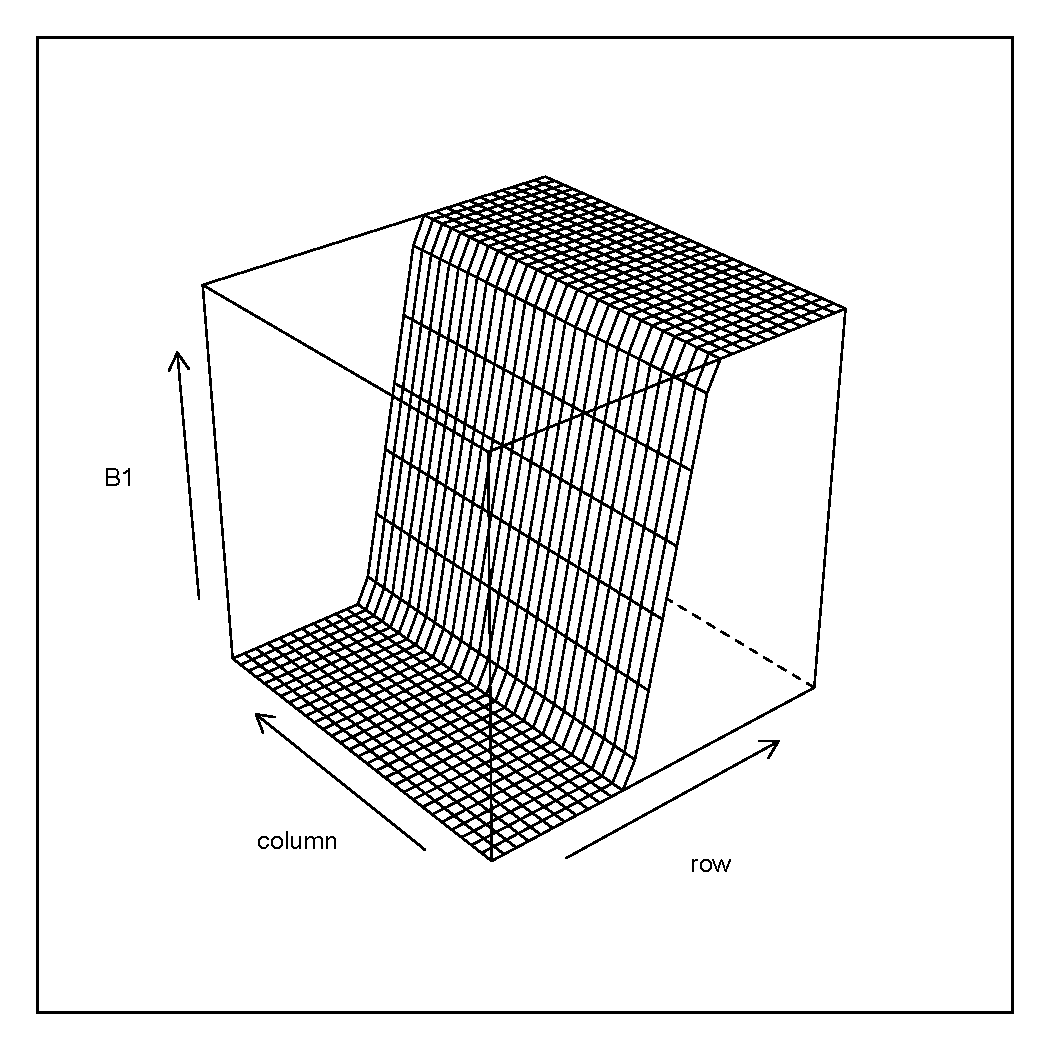
\includegraphics[width=0.32\textwidth]{../../figures/simulation/step.pdf}
			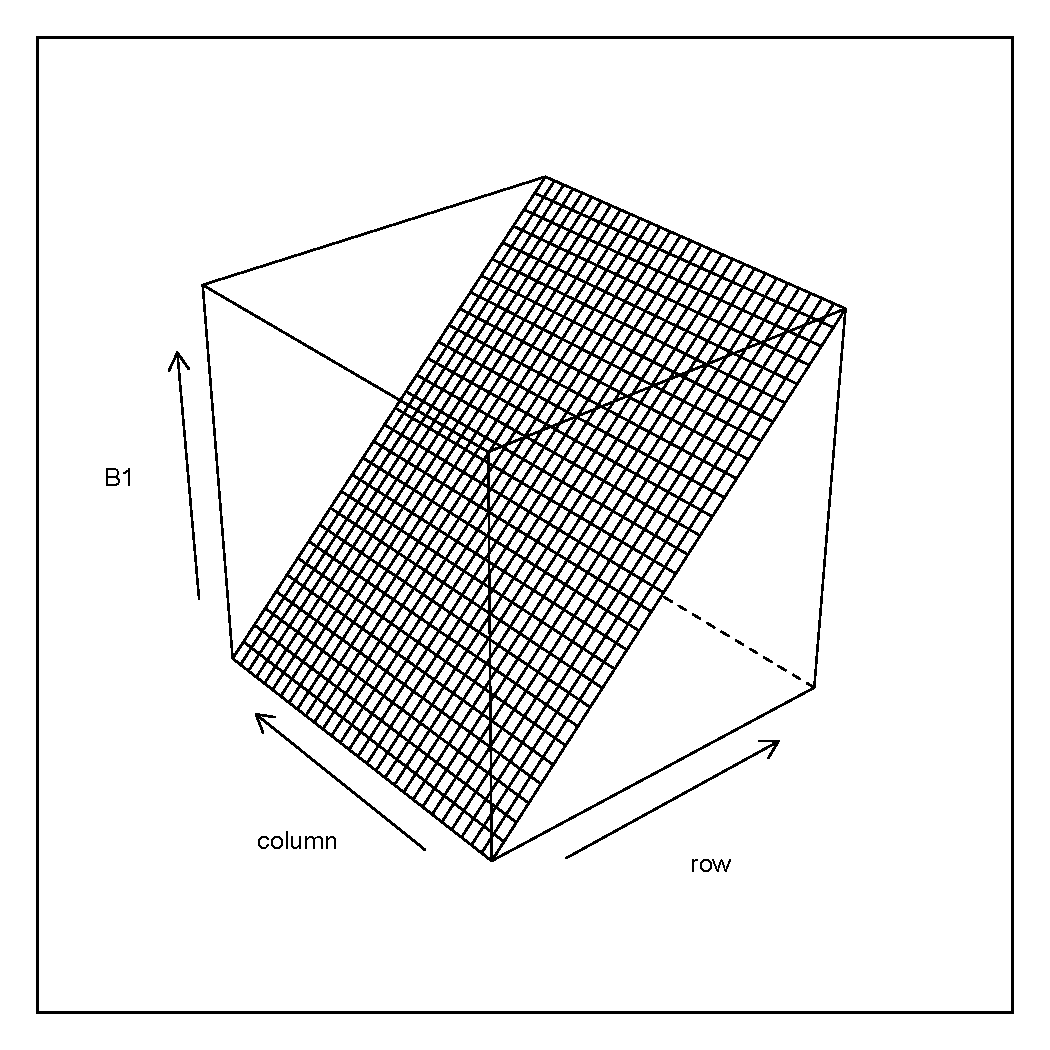
\includegraphics[width=0.32\textwidth]{../../figures/simulation/gradient.pdf}
			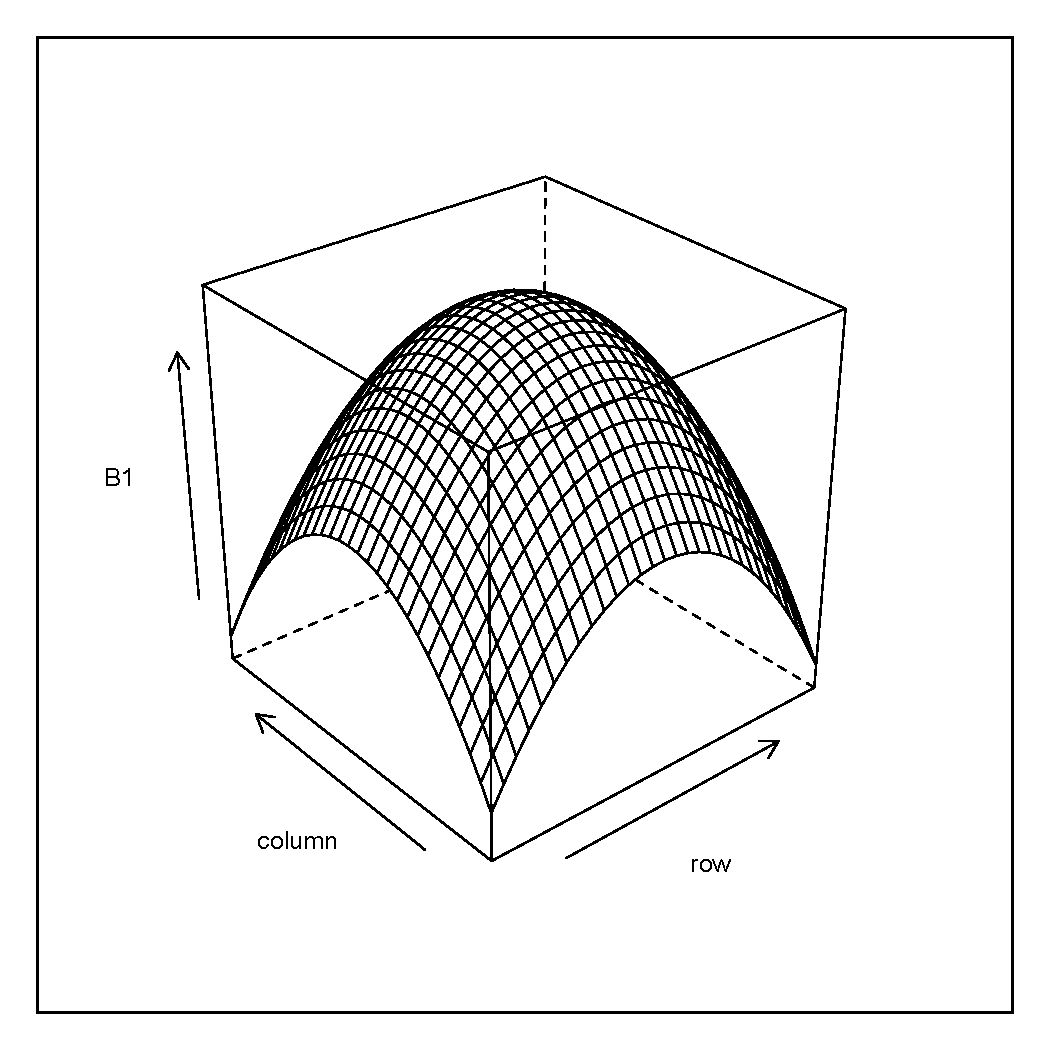
\includegraphics[width=0.32\textwidth]{../../figures/simulation/parabola.pdf}
			\caption{The actual $\beta_1$ coefficient surface used in the simulation.\label{fig:sim-actual}}
		\end{center}
	\end{figure}
	
	\begin{figure}
		\begin{center}
			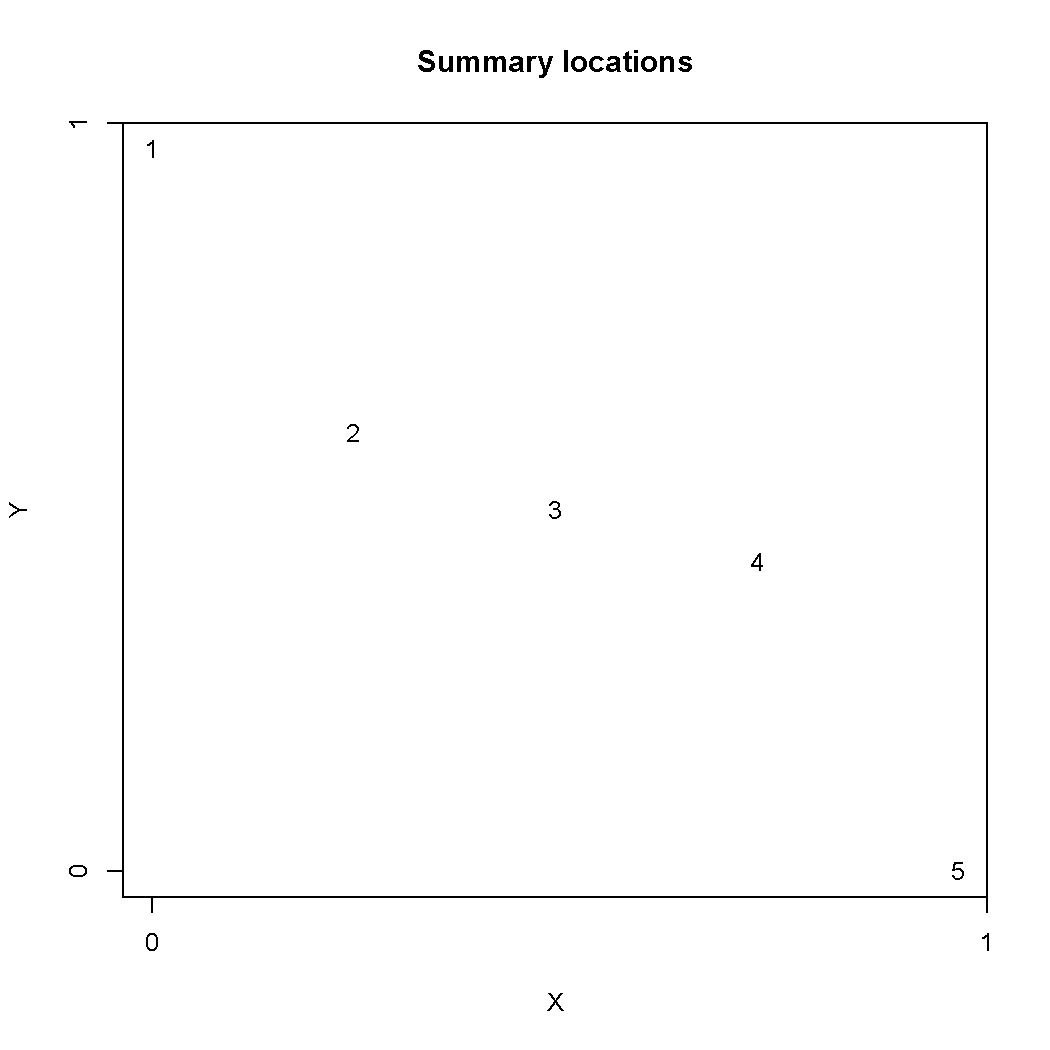
\includegraphics[width=0.5\textwidth]{../../figures/simulation/summary-locations.pdf}
			\caption{Locations where the variable selection and coefficient estimation of GWL were summarized.\label{fig:summary-locations}}
		\end{center}
	\end{figure}
	
	\paragraph{Summary locations}Results of the simulation were summarized at five locations on the domain (Figure \ref{fig:summary-locations}). Due to edge effects, we expect biased estimation at locations one and five (which are at opposite corners of the domain) from traditional GWR, particularly when the coefficient surface has nonzero gradient at the boundary (which is the case for the gradient and parabola functions). Because the GWEN and oracular GWR use locally linear fitting, they are expected to exhibit less bias at the boundaries.
	
	Locations two and four are at the `corners' of the step function. Because the step function is undifferentiable at these locations, locally linear fitting is not expected to be as effective at reducing bias here as at the boundaries of the gradient and parabola functions.
	
	Local variable selection is expected to be ambiguous at locations where the underlying coefficient surface transitions from zero to nonzero. In the simulations, that occurs at location four of the step function, location five of the gradient, and locations one and five of the parabola.
	
	Unlike the other two functions, the gradient is actually constant across the domain in terms of the covariate-by-location interaction. As a result, the optimal kernel bandwidth $\phi$ is expected to be larger for estimating the gradient coefficient surface than for the step or the parabola. The result should be that the estimation is more accurate for the gradient function in terms of bias, variance, and MSE.
		
	\subsection{Simulation results}	
	\paragraph{Selection} Table \ref{table:selection} lists the results of variable selection. The correct covariate was usually included in the local models, and the unimportant covariates were usually excluded. Ignore for now the ambiguous locations where the true $\beta_1$ surface transitions from zero to nonzero. Of the eighty simulated cases where $\beta_1(\bm{s})$ is unambiguously nonzero, more than half (59) saw no false negatives (over 100 simulations). The number with no false negatives and no false positives (i.e. exactly the correct model was recovered in all 100 simulations) was 44. Of the 120 total simulated cases, 72 had no false positives (i.e. no variable whose true coefficient is zero was included in the model during any of the 100 simulation runs). 
	
	Selection performance was more affected by an increase in the noise variance from $\sigma^2_{\varepsilon}=0.25$ to $\sigma^2_{\varepsilon}=1$ than by an increase in colinearity from $\rho = 0$ to $\rho = 0.5$. Of the 44 cases where model selection recovered exactly the correct model in all 100 runs of the simulation, only five arose from cases where $\sigma^2_{\varepsilon}=1$, while 19 arose from cases where $\rho = 0.5$. The worst error rates that were observed in these unambiguous cases were a false positive rate of 6\% (location one of the step function with $\sigma^2_{\varepsilon}=1$, $\rho=0.5$, and selection via the elastic net) and a false negative rate of 16\% (location three of the step function with $\sigma^2_{\varepsilon}=1$, $\rho=0.5$, and selection via the lasso).
			
	Model selection was ambiguous at locations where the true $\beta_1(\bm{s})$ transitions from zero to nonzero. At location four of the step function, the selection rate of $\beta_1$ ranged from 43\% to 60\% among the different simulation settings. At location five of the gradient, the range of selection rates was 63\% to 82\%, and the selection rate across locations one and five of the parabola ranged from 27\% to 66\%. 

	There is no indication that the GWEN performed better in selection than the GWAL, even in cases where the covariates were moderately correlated ($\rho=0.5$).
	
	\paragraph{Coefficient Estimation} The mean squared error, bias, and variance of $\hat{\beta}_1$ (MSE$(\beta_1)$, bias$(\hat{\beta}_1)$, var$(\hat{\beta}_1)$) are listed in Tables \ref{table:msex}, \ref{table:bx}, and \ref{table:varx}, respectively. The method of oracular selection led to the best MSE$(\hat{\beta}_1)$ in 41 of the 60 cases.
	
	In terms of MSE$(\hat{\beta}_1)$, while oracular selection clearly was the most accurate estimation method in most cases, the difference in accuracy between the estimation methods was modest in most cases. There were a few cases when the difference in MSE$(\hat{\beta}_1)$ between estimation methods amounted to at least an order of magnitude. At locations one and five of the parabola, oracular selection produces much more accurate estimation than GWEN, GWAL, or GWR because locations one and five are on the domain boundary where the parabola has a strong gradient, and those methods don't use locally linear fits to account for the boundary effect. This can also be seen from the fact that the bias$(\beta_1)$ of {\tt enet}, {\tt lasso}, and {\tt gwr} is large at locations one and five of the parabola, where it is nearly zero for {\tt u.lasso}, {\tt u.enet}, and {\tt oracular}.
	
	A similar boundary effect is apparent at location five of the gradient, where GWEN, GWAL, and GWR produce a bias$(\hat{\beta}_1)$ and MSE$(\hat{\beta}_1)$ that are an order of magnitude or more greater than those of {\tt u.lasso}, {\tt u.enet}, and {\tt oracular} (the differences in var$(\hat{\beta}_1)$ are smaller).
	
	At location one of the step function, the MSE$(\beta_1)$ and var$(\beta_1)$ for {\tt gwr} are much smaller than for the other estimation methods, including {\tt oracular}, while the bias$(\beta_1)$doesn't vary much between estimation methods. It is not clear why this is the case.
		
	As was the case for selection, accuracy in coefficient estimation seemed to suffer more from an increase in the noise variance than from increased correlation in the covariates. Once again, this effect is probably most apparent at location three of the step function.
	
	
	
	\paragraph{Fitted Values} The MSE of the $\hat{Y}$, $\text{MSE}\left(\hat{Y}\right)$, is listed in Table \ref{table:msey}. Nominally, $\text{MSE}\left(\hat{Y}\right)$ should be equal to the noise variance, $\sigma_{\varepsilon}^2$, which is 1 for odd-numbered rows and 0.25 for even numbered rows. Of the 60 simulation cases, {tt gwr} produced the minimal residual variance for 22, which is more than any other method. Where the residual noise 
	
	\input{../../output/simulation/selection}
	\input{../../output/simulation/msex}
	\input{../../output/simulation/bx}
	\input{../../output/simulation/varx}			
	\input{../../output/simulation/msey}

			
\section{Data Analysis\label{section:data-analysis}}
	An example data analysis is presented to demonstrate application of the GWEN for local variable selection in an SVCR model of how poverty is related to a list of socio-economic variables.
	
	\subsection{Census Poverty Data}
	An example demonstrates application of the GWEN to the identification of socio-economic covariates that are locally meaningful predictors of the county-level poverty rate in the upper midwestern states of Minnesota, Iowa, Wisconsin, Illinois, Indiana, and Michigan. The data used in this example are aggregated at the level of counties, which are areal units. Each county's centroid is treated as its sampling location. The data came from the U.S. Census Bureau's decennial census in the year 1970.
	
	Three kinds of variables  were considered as potential predictors of county-level poverty rate.
	\begin{itemize}
		\item Covariates that describe the county's employment structure ($\verb!pag!$, the proportion of residents employed in agriculture, $\verb!pex!$, the proportion of residents employed in mining, $\verb!man!$, the proportion of residents employed in manufacturing, $\verb!pfire!$, the proportion of residents employed in finance, insurance, and real estate, $\verb!pserve!$, the proportion of residents employed in services, and $\verb!potprof!$, the proportion of residents employed in other professions)\\
		\item Covariates that describe the county's racial makeup ($\verb!pwh!$, the proportion of residents who are white, $\verb!pblk!$, the proportion of residents who are black, and $\verb!phisp!$, the proportion of residents who are hispanic)\\
		\item $\verb!pmetro!$: an indicator of whether the county is in a metropolitan area.
	\end{itemize}
	The response variable (poverty rate) is a proportion, taking values in $[0,1]$. To demonstrate the geographically-weighted Lasso in a linear regression context, we model the logit-transformed poverty rate. The predictor variables were not transformed - raw proportions were used.
	
	\subsection{Modeling}	
	The AEN was used for variable selection, and then coefficients for the selected variables were estimated by weighted least squares without shrinkage. The standard {\tt gwr} algorithm was used to fit a model to the same data for the sake of comparison.
	
	\subsection{Figures}
	The coefficient estimates are plotted on maps of the upper midwest in Figure \ref{fig:unshrunk-enet-coefs-1970} (based on the AEN) and Figure \ref{fig:gwr-coefs-1970} (for traditional GWR).
	\begin{figure}
		\begin{center}
			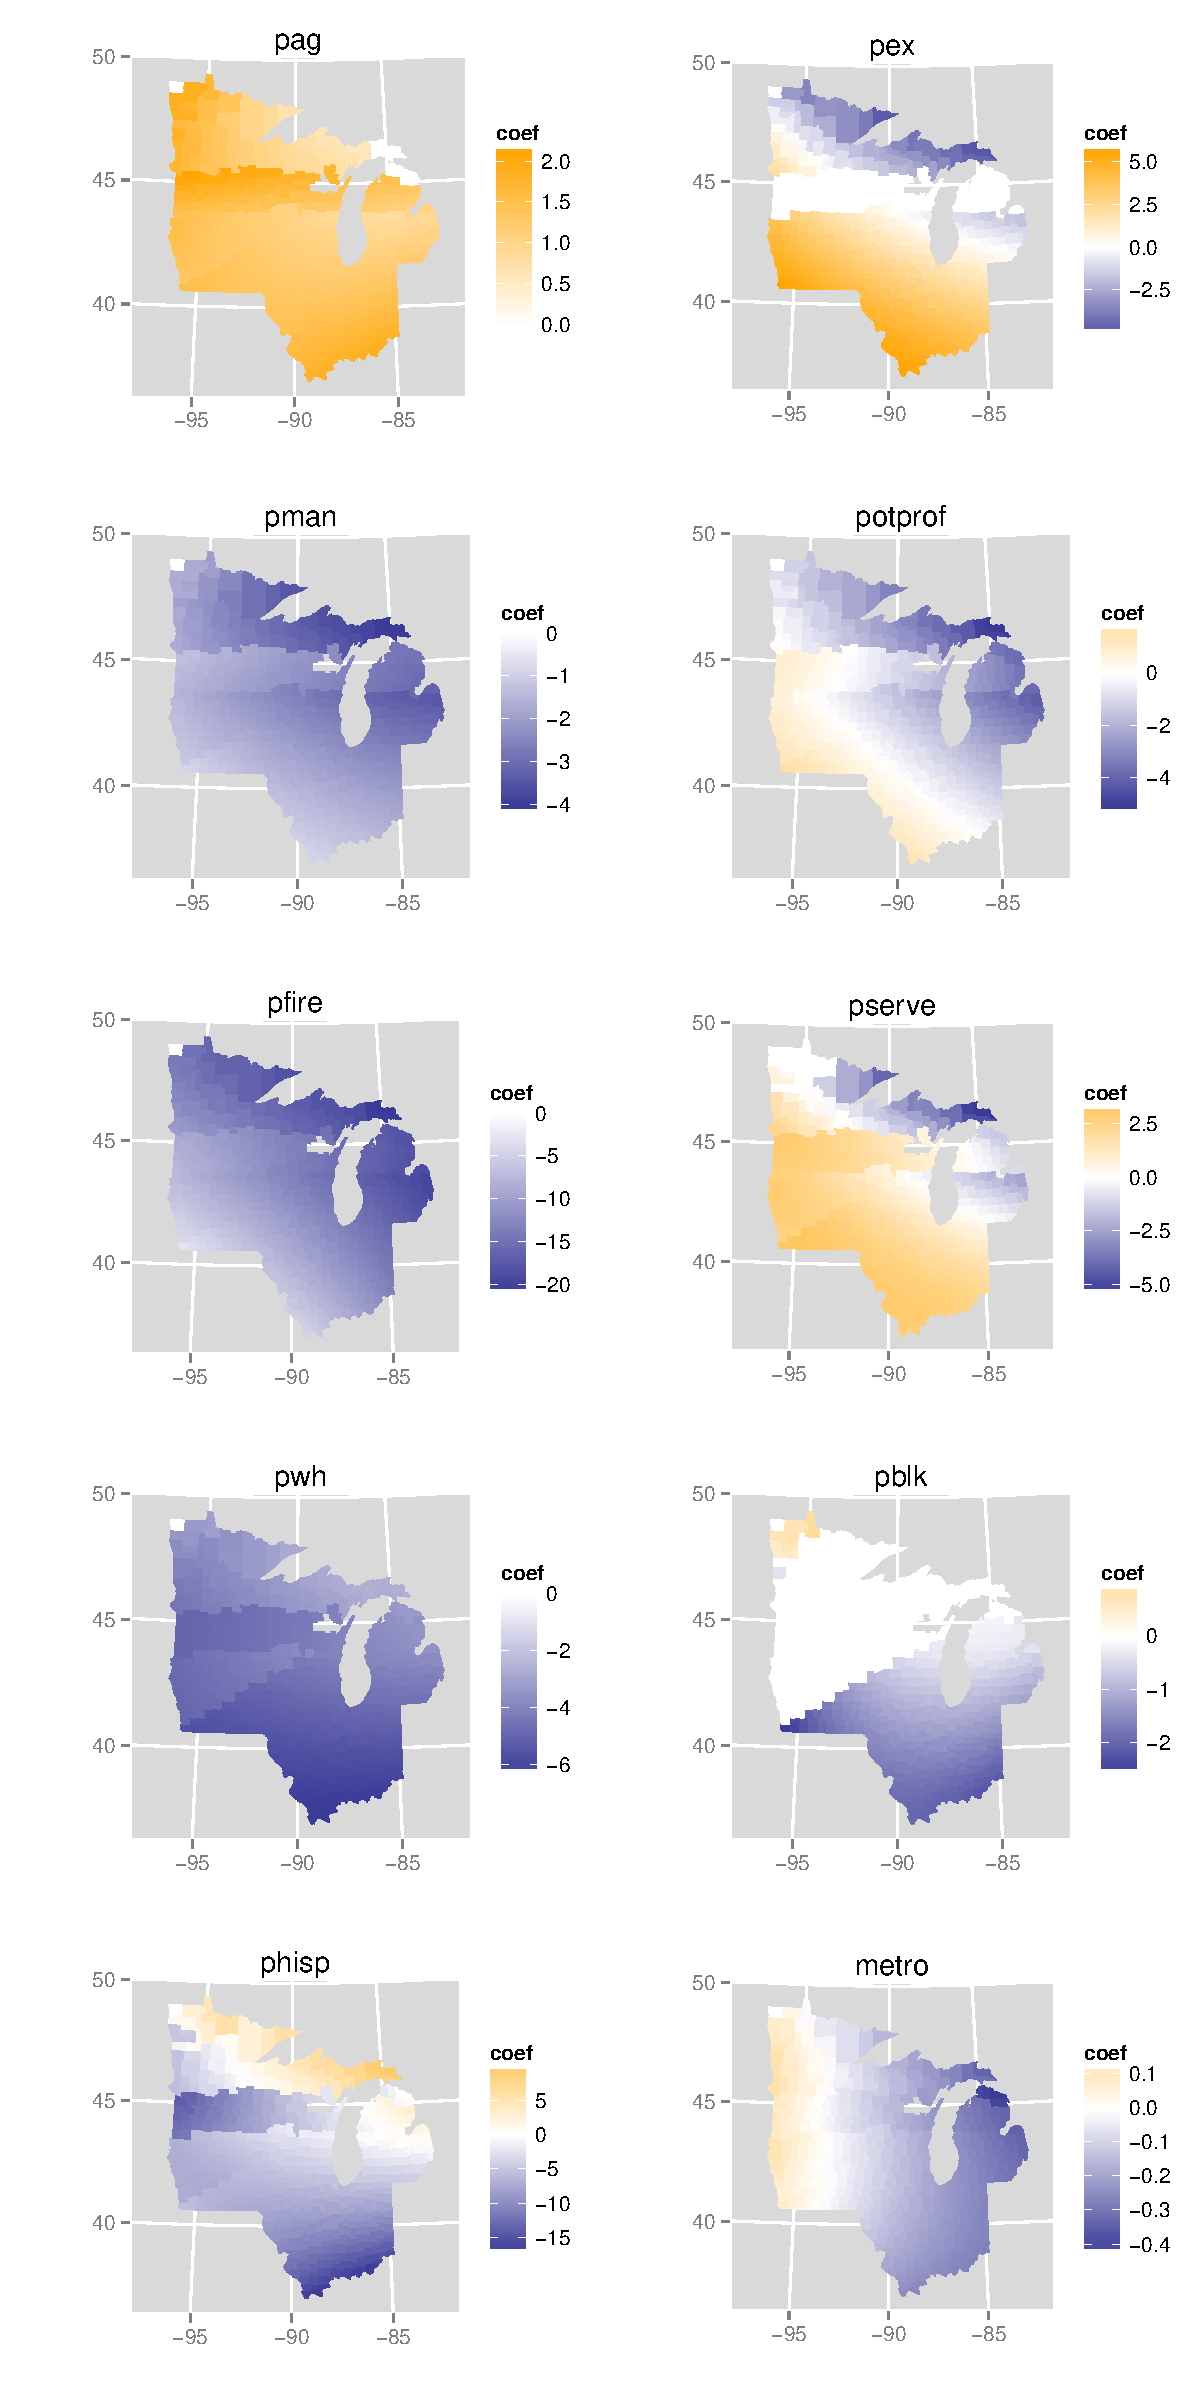
\includegraphics[height=8in]{../../figures/poverty/1970-enet-linear-coefficients-unshrunk.pdf}
			\caption{Coefficient surfaces for the logit of poverty rate, based on the 1970 census and selected by the GWEN. \label{fig:unshrunk-enet-coefs-1970}}
		\end{center}
	\end{figure}	
		
	\begin{figure}
		\begin{center}
			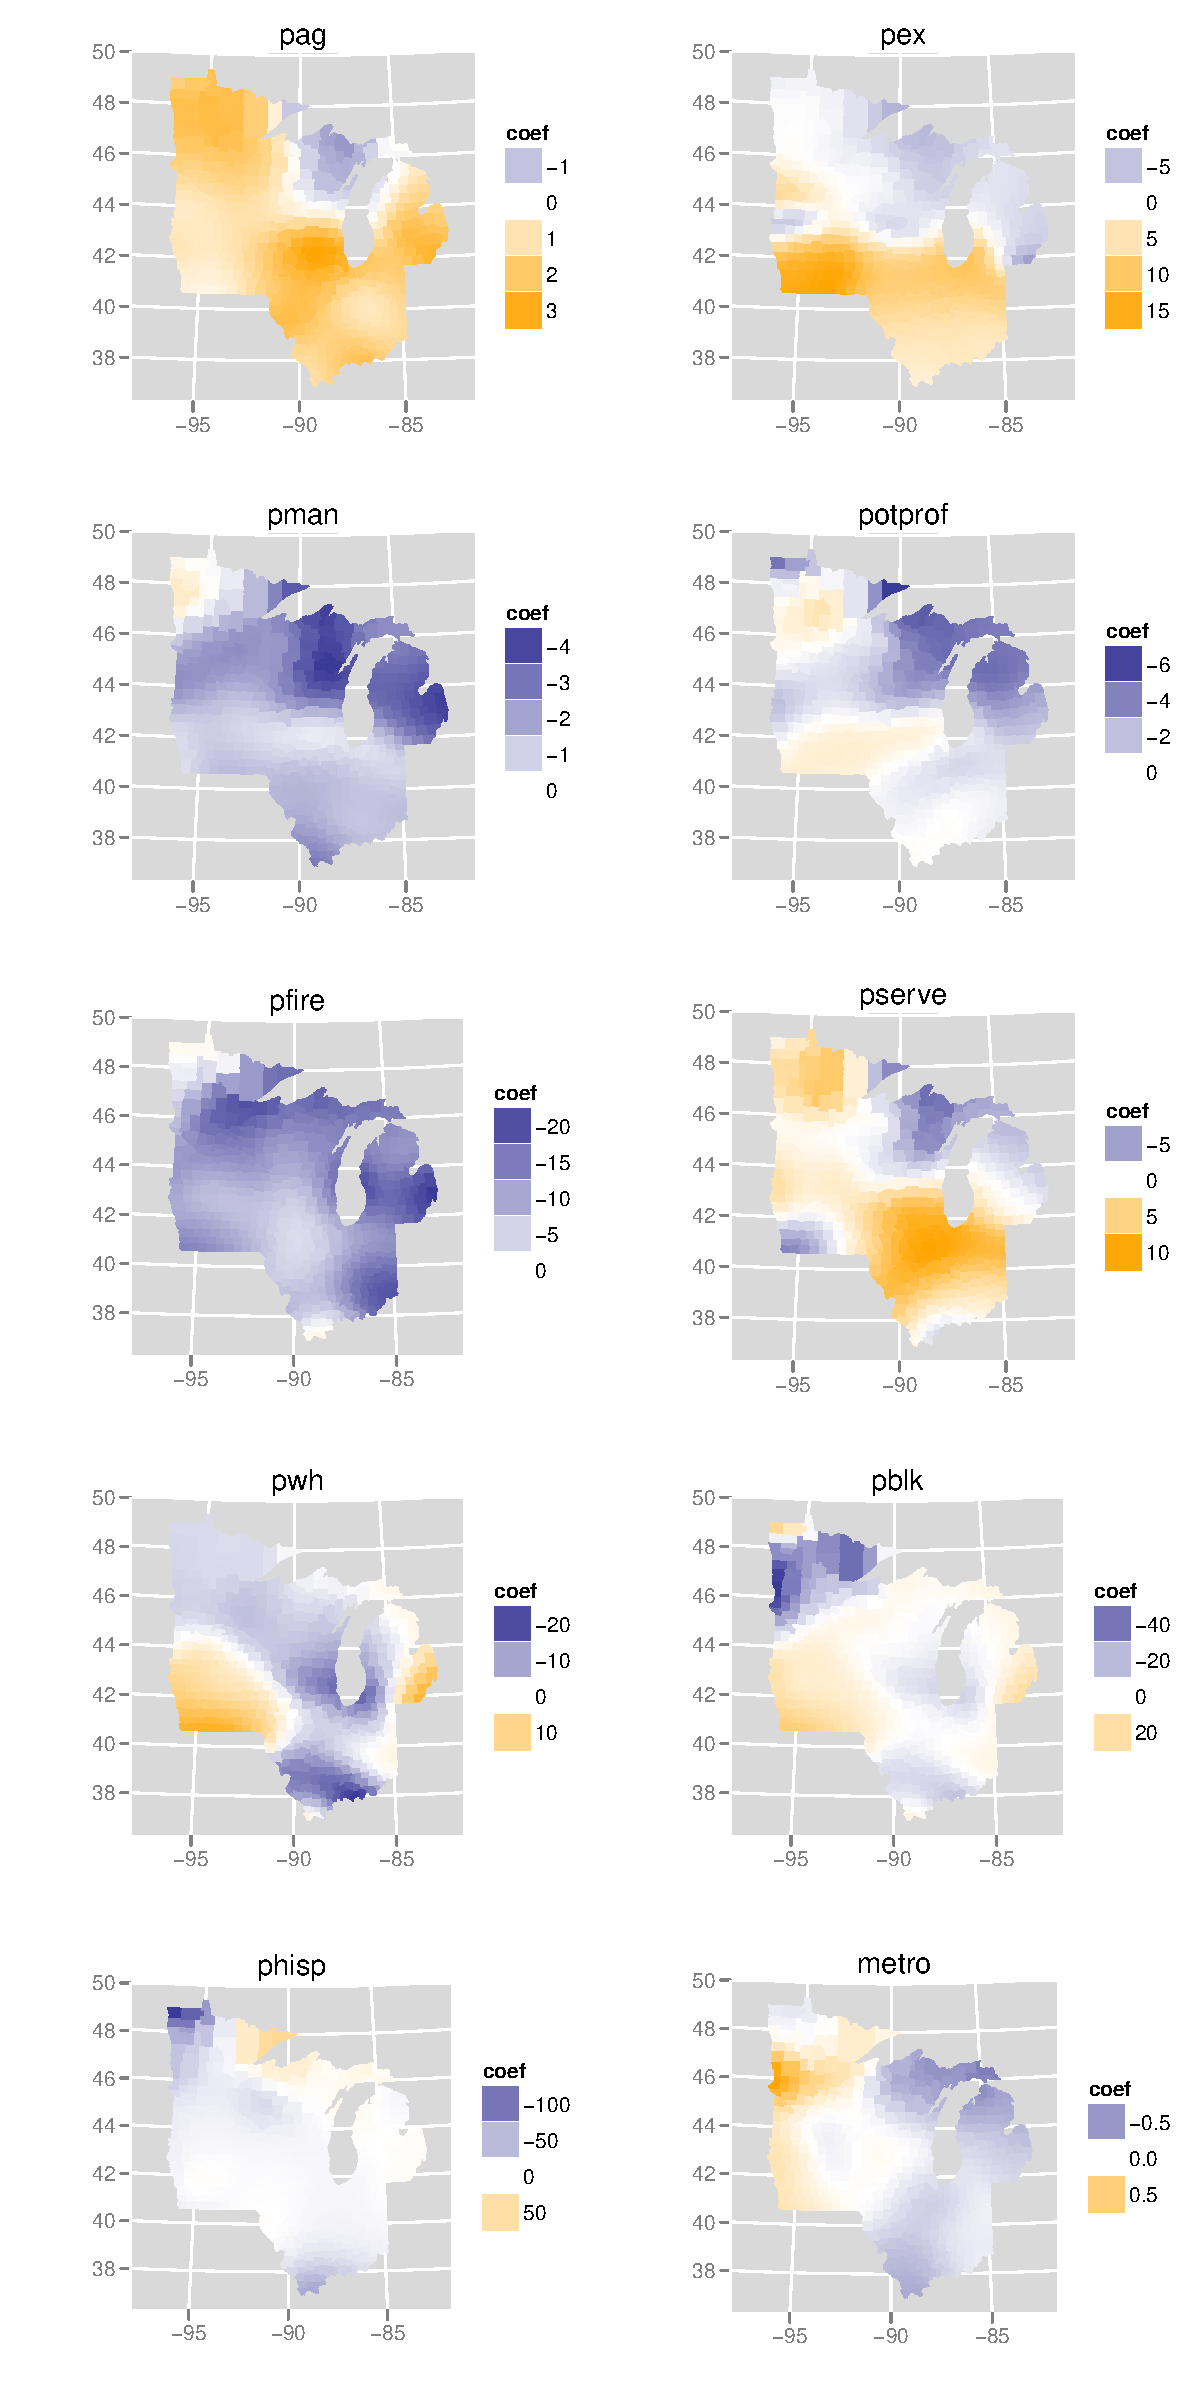
\includegraphics[height=8in]{../../figures/poverty/1970-gwr.pdf}
			\caption{Coefficient surfaces for the logit of poverty rate based on the 1970 census and estimated by traditional GWR. \label{fig:gwr-coefs-1970}}
		\end{center}
	\end{figure}
			
	\subsection{Discussion}
	It is immediately apparent that the estimated coefficient surfaces are non-constant for most variables. The same large-scale patterns appear in both figures, but with differences. First of all, the AEN has selected a larger bandwidth than traditional GWR, so there is less variability in the coefficient estimates from the AEN. This may be one reason that the AEN coefficient estimates are less extreme than those for traditional GWR. In a model with a logit-transformed proportion as the output, the coefficients can be interpreted as log odds ratios, so, e.g., the estimate of -100 as the coefficient of \verb!phisp! (albeit at the edge of the domain) seems unrealistic.
	
	Assessing variable selection for this data is difficult, since the AEN almost never removed any variables from the model. Indeed, some coefficients seem nearly constant across the domain. An exception is the coefficient surface for \verb!pex! (mining employment). That surface indicates an interaction whereby the proportion of people working in mining in southern parts of the domain is associated with an increase in the poverty rate, while in northern parts of the domain it is associated with a decrease in the poverty rate.


\section{Future work \label{section:future-work}}
	The GWEN is presented here as a method of analysis for data where the response variable follows a gaussian distribution with independent additive errors. A key feature of spatial data, though, is that the errors are typically autocorrelated. Additionally, it is common to encounter data that does not follow a gaussian distribution but for which the GWEN would otherwise be a valuable tool for analysis.

	\paragraph{Autocorrelated Errors} In order to get a sense of how the GWEN will perform when the assumption of independent errors is violated, the simulation study from Section \ref{section:simulation} was repeated with the addition of a Mat\`{e}rn-class spatial covariance structure in the noise (results not included here). Introducing autocorrelation in the errors causes a substantial degradation in the estimation accuracy of the GWAL and GWEN, accompanied by a tendency to prefer smaller kernel bandwidths. The likely explanation is that when the kernel bandwidth is small, autocorrelated errors are indistinguishable from a varying intercept. The residuals are reduced to the extent that the errors are incorporated in the intercept term. Since this effect is absent in the case of uncorrelated errors, greater autocorrelation in the error term will tend to mean a greater reduction in the errors - and therefore a greater increase in the log likelihood - as the kernel bandwidth decreases.
	
	Since the optimal kernel bandwidth is balance between the log likelihood and the degrees of freedom consumed by the model, and because the effect of autocorrelated errors is an increase in log likelihood without an offsetting increase in the consumed degrees of freedom at a given kernel bandwidth, greater autocorrelation will tend to lead to a smaller optimal kernel bandwidth. One quick way to counter this effect is to increase the penalty that is added to the total log likelihood in (\ref{eq:AICc}). There is currently no rule to set the penalty based on the data, which would be necessary before using this adjustment to analyze real data.
	
	\paragraph{Generalized linear models} To date, validation of the GWEN has been for gaussian data. The extension to any exponential-family distribution involves generalizing the likelihood that is used to select AEN tuning parameters and the kernel bandwidth. Preliminary simulations of the generalized GWEN have been carried out with Poisson and binomial data.

\section{References}
\bibliographystyle{chicago}
\bibliography{../../references/gwr}

\end{document}  